\chapter{Resultados e Discussão} \label{cap:resultados}

As arquiteturas descritas no capitulo \ref{cap:modelagem} foram treinadas durante as 10 primeiras épocas para os valores de $l_r$ = $10^{-\eta}$, com $\eta=1,2,3,4,5$. Os resultados análise são apresentados no inicio deste capítulo. Posteriormente, o comportamento das redes treinadas por mais épocas é explicitado. Ao fim, apresentamos nossas conclusões sobre o estudo.

\section{Dinâmica Inicial}

Na tabela \ref{tab:modelos_iniciais} vemos o tamanho, o tempo médio na fase de treino e o tempo médio total por época de arquiteturas selecionadas. O desvio padrão relativo é menor do que $0.1\%$ em todas as médias. Em geral, a etapa de treino constitui de $70\%$ à $85\%$ do tempo total de uma época.

\begin{table}[ht]
	\begin{center}
		\caption{Comparação do tempo de treino entre as arquiteturas.}
		\label{tab:modelos_iniciais}
		\begin{tabular}{ |c|c|c|c| }
			\hline
			modelo & 
			\begin{tabular}[c]{@{}c@{}}tamanho\\ (parâmetros)\end{tabular} & \begin{tabular}[c]{@{}c@{}}$\tilde{\tau}$\\(segundos) \end{tabular}& \begin{tabular}[c]{@{}c@{}}$\tau$\\ (segundos)\end{tabular}\\ \hline\hline
			% RMch
			(a) $M$ & $5.4\,10^{6}$  & $72.63$ & $100.97$ \\ \hline
			
			% RMchD
			(b) $MD$ & $5.4\,10^{6}$ & $75.96$ & $108.14$ \\ \hline
			
			% C5o6RMch
			(c) $C_6M$ & $2.4\,10^{6}$ & $66.96$ & $91.24$ \\ \hline
			
			% C5o6RMchD
			(d) $C_6MD$ & $2.4\,10^{6}$ & $71.19$ & $97.57$ \\ \hline
			
			% C5o6C5o12RMchD
			(e) $C_6C_{12}MD$ & $4.4\,10^{6}$ & $238.66$ & $291.03$ \\ \hline
			
			% C5o6C5o12Rfl100MchD
			(f) $C_6C_{12}Fl_{100}MD$ & $2.4\,10^{6}$ & $311.42$ & $357.51$ \\ \hline
			
			% C5o6C5o12C5o36C5o36RMchD
			(g) $C_6C_{12}C_{36}C_{36}MD$ & $4.5\,10^{5}$ & $249.53$ & $302.44$ \\ \hline
			
			% C5o6C5o12C5o36C5o36Rfl100MchD
			(h) $C_6C_{12}C_{36}C_{36}Fl_{100}MD$ & $2.9\,10^{5}$ & $256.97$ & $308.77$ \\ \hline
			
			Pinto\cite{otaro} & 6.9 $10^{7}$ & - & - \\ \hline
		\end{tabular}\hfill%
	\end{center}
\end{table}

A partir da tabela podemos ver que o tempo consumido depende não apenas da quantidade de parâmetros, mas também da arquitetura. As arquiteturas $C_6M$ e $C_6C_{12}Fl_{100}MD$, por exemplo, possuem aproximadamente o mesmo número de parâmetros, sendo a última, entretanto, pelo menos quatro vezes mais lenta. Em todas as arquiteturas estudadas, a adição do dropout aumentou o ligeiramente o tempo de treino (entre $3\%$ e $10\%$), mostrando-se uma operação computacionalmente barata. Camadas de maxpooling (omitidas da tabela por brevidade), entretanto, mostraram-se computacionalmente custosas, aumentando a demanda de tempo em pelo menos duas vezes. Chamamos a atenção de que a relação entre as camadas é tão importante para o tamanho e tempo de execução quanto a especificação da camada em sí. No par (d)-(e), por exemplo, a adição de uma camada convolucional aumentou consideravelmente o tamanho e o tempo de execução. Nesse caso, os canais extras adicionados aumentaram substancialmente a camada densa seguinte. No par (e)-(f) a camada densa reduz drasticamente a quantidade de sinais (de 24192 para 100), reduzindo o tamanho da entrada da camada multi-caractere seguinte, adicionando, entretanto, uma maior de demanda de tempo. Em geral, podemos estabelecer que camadas densas normalmente demandam mais tempo, enquanto camadas convolucionais, usualmente reduzem o número de sinais e tamanho total da arquitetura, mas o impacto exato precisa ser estimado à luz das demais camadas. Para comparação, o modelo no estudo de pinto possui, aproximadamente, $13$ vezes o tamanho do maior e 250 vezes o do menor modelo proposto no presente estudo.   

\begin{figure}[!p]
	\begin{center}
		\caption{Dinâmica inicial de arquiteturas selecionadas.}\label{loss_val}
		\begin{subfigure}{.5\textwidth}
			\centering
			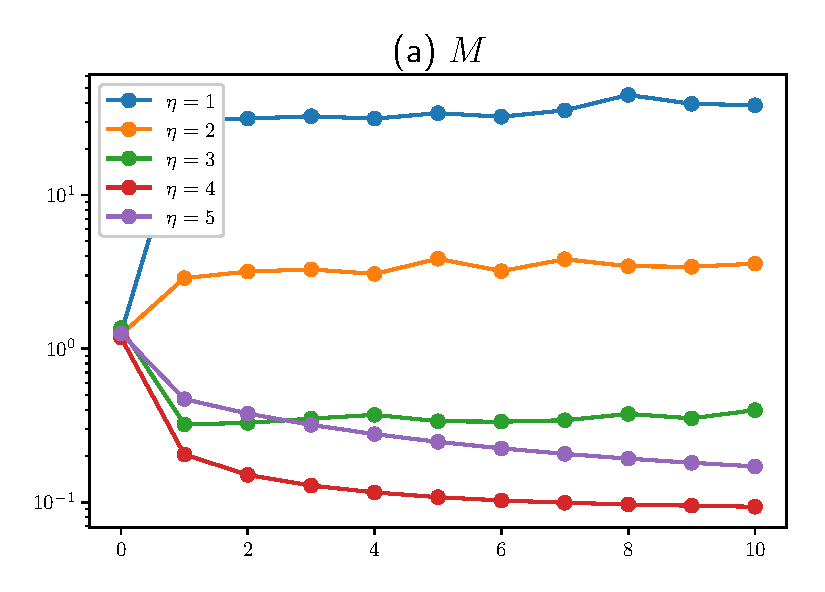
\includegraphics[width=0.95\linewidth]{figuras/RMch.eps}
		\end{subfigure}\hfill%
		\begin{subfigure}{.5\textwidth}
			\centering
			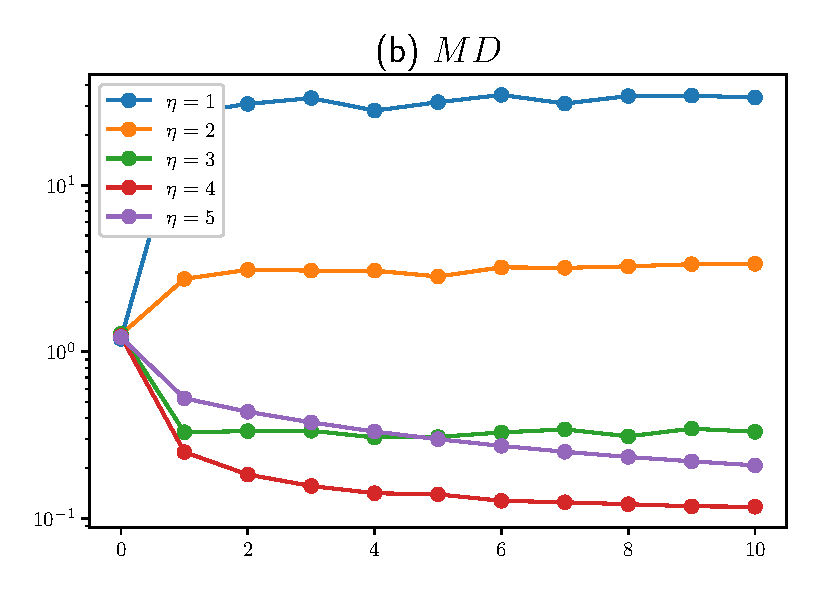
\includegraphics[width=0.95\linewidth]{figuras/RMchD.eps}
		\end{subfigure}\hfill%
		\newline
		\begin{subfigure}{.5\textwidth}
			\centering
			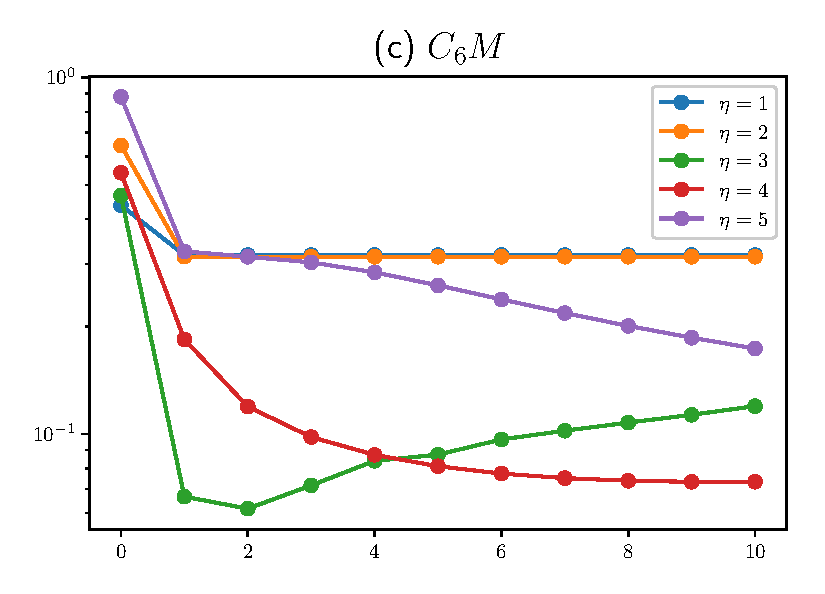
\includegraphics[width=0.95\linewidth]{figuras/C5o6RMch.eps}
		\end{subfigure}\hfill%
		\begin{subfigure}{.5\textwidth}
			\centering
			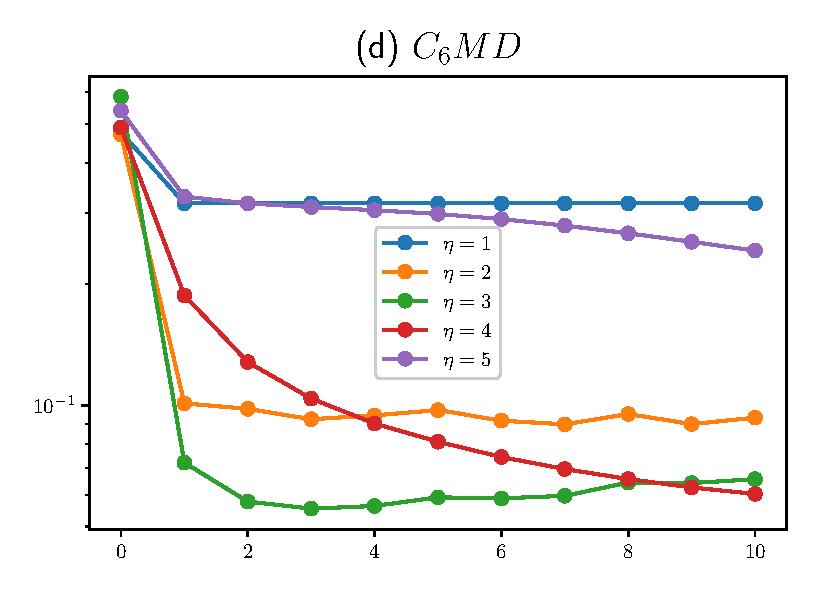
\includegraphics[width=0.95\linewidth]{figuras/C5o6RMchD.eps}
		\end{subfigure}\hfill%
		\newline\hspace*{-0.2cm}\makebox[0cm]{\rotatebox{90}{\hspace*{2.5cm}$log \left(  J^{(D_{val})}  \right) $\hspace*{-2.5cm}}}\hspace*{0.2cm}%
		\begin{subfigure}{.5\textwidth}
			\centering
			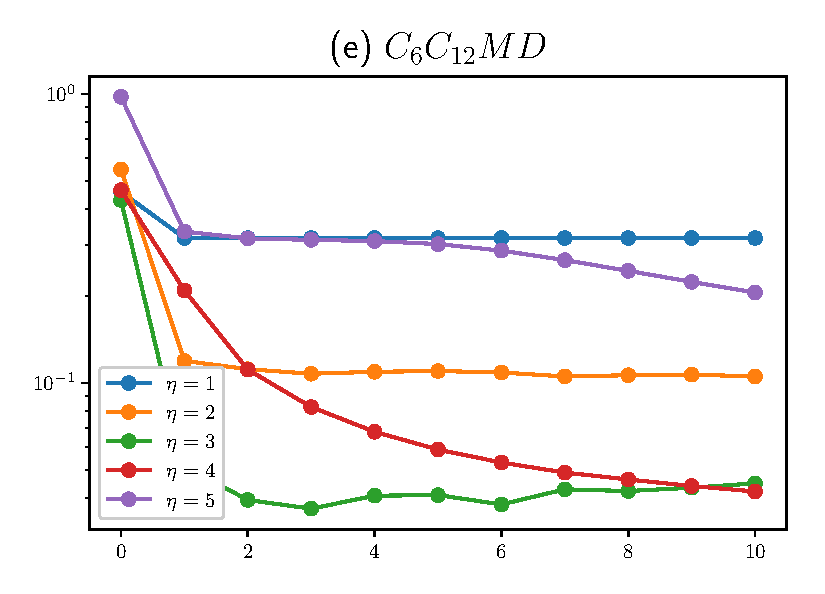
\includegraphics[width=0.95\linewidth]{figuras/C5o6C5o12RMchD.eps}
		\end{subfigure}\hfill%
		\begin{subfigure}{.5\textwidth}
			\centering
			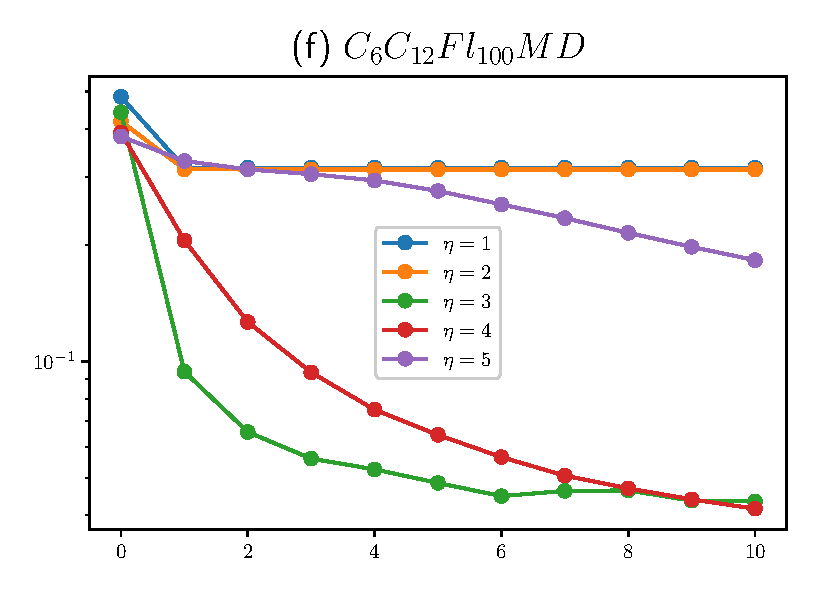
\includegraphics[width=0.95\linewidth]{figuras/C5o6C5o12Rfl100MchD.eps}
		\end{subfigure}
		\newline
		\begin{subfigure}{.5\textwidth}
			\centering
			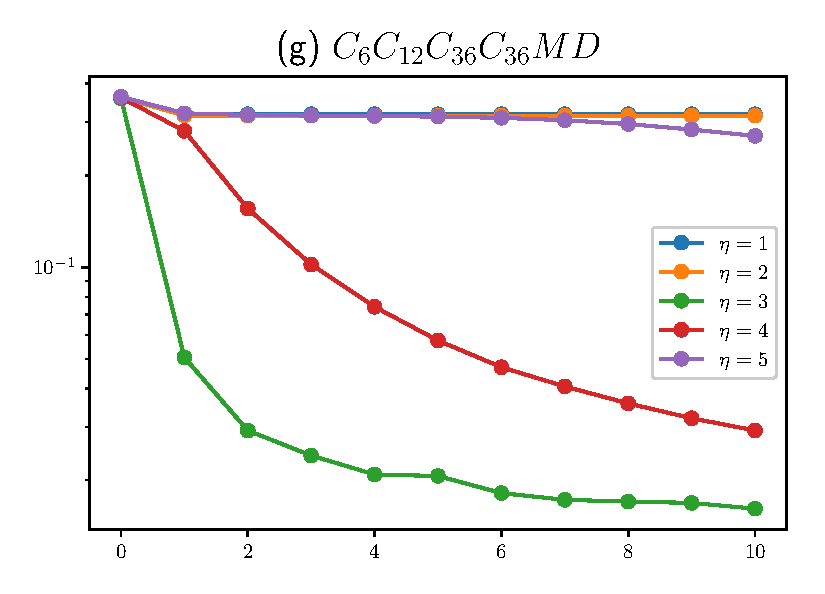
\includegraphics[width=0.95\linewidth]{figuras/C5o6C5o12C5o36C5o36RMchD.eps}
		\end{subfigure}\hfill%
		\begin{subfigure}{.5\textwidth}
			\centering
			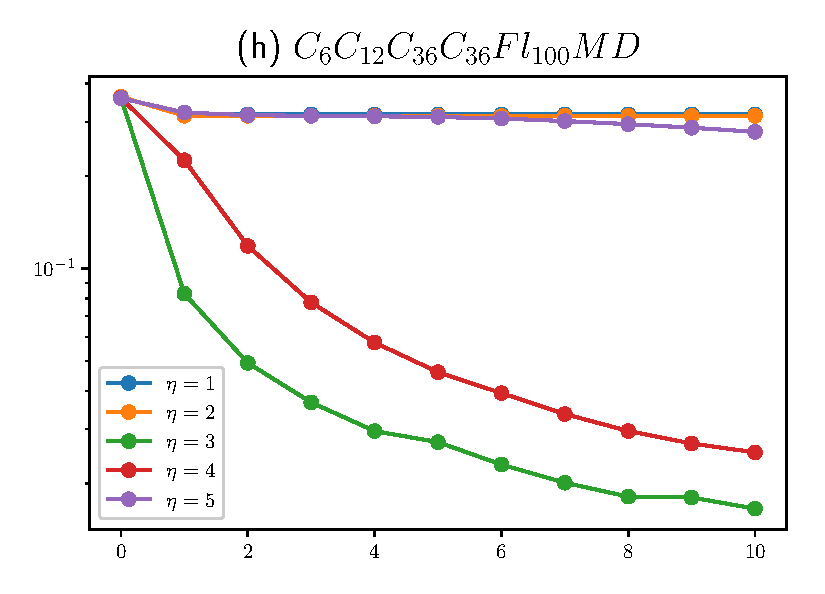
\includegraphics[width=0.95\linewidth]{figuras/C5o6C5o12C5o36C5o36Rfl100MchD.eps}
		\end{subfigure}\hfill%
		\newline
		$t$ (épocas)
	\end{center}
	\small Nos gráficos apresentamos a função custo na escala logarítmica de modo a facilitar a visualização. Os traços são apenas guias visuais. As arquiteturas estão indicadas nos títulos em correspondência com a tabela \ref{tab:modelos_iniciais} e os valores do hiper-parâmetro de aprendizado estão indicados na legenda.
\end{figure}

Na figura \ref{loss_val} podemos ver a evolução da função custo no conjunto de validação durante as 10 primeiras épocas para diferentes arquiteturas de rede e valores $\eta=1,2,3,4,5$. Para $\eta=1$ e $\eta=2$, vemos que o custo atinge um platô já durante as primeiras épocas da dinâmica. A estagnação em $J$ é um indicativo de que as correções para o gradiente da função de custo cresce de forma descontrolada. Quando isso ocorre, o algoritmo adaptativo Adam tende a anular as atualizações em subespaços de $\{\Theta\}$, atualizando os parâmetros apenas nas direções de maior gradiente de $J$. Isto ocorre porque, antes das atualizações, o algoritmo normaliza $\nabla_{\Theta} J$ pelo módulo do gradiente acumulado nos últimos lotes. Assim, se $|\nabla_{\Theta} J| \rightarrow \infty$, $\Delta \Theta \rightarrow 0$, exceto nas regiões onde o gradiente é proporcional acumulado do seu módulo. Em outras palavras, o algoritmo superestima o erro em uma determinada direção um detrimento das demais. Isso leva a rede a cometer os mesmos erros repetidamente nas direções não atualizadas. É importante ressaltar que em algoritmos onde essa normalização não é aplicada (como o \textit{método do gradiente}, por exemplo), quando esse fenômeno ocorre, o valor do custo e os parâmetros também crescem de forma descontrolada. A dinâmica da função de custo nas redes $M$ e $MD$ corroboram para essa interpretação. No gráfico dessas arquiteturas podemos observar um aumento significativo no valor de $J$ antes das atualizações cessarem. Para uma análise mais precisa teríamos de acompanhar a evolução $\Theta$ ao longo do treino, o que esta fora do escopo do presente trabalho. No outro extremo, $\eta=5$, vemos um comportamento similar durante as épocas iniciais para algumas arquiteturas (c-h). Entretanto, a aparente estagnação nesses casos é devida à lenta convergência induzida por esse valor do hiper-parâmetro, observando-se uma melhoria no valor de $J$ na sequência da dinâmica. Assim, esses valores definem os limites práticos para a busca do melhor hiper-parâmetro de aprendizado neste problema.

O valor $\eta = 4$ exibe as dinâmicas mais estáveis, onde a função de custo apresenta um comportamento monotonicamente decrescente durante toda dinâmica, eventualmente estagnando, como visto em (a-d). Para as demais redes (e-i) nota-se que o valor da função de custo ainda apresentaria melhoras caso continuássemos a evolução por mais épocas. Para $\eta = 3$, vemos que a dinâmica é, de fato, mais rápida nas arquiteturas (c-i). Contudo, esse valor leva a instabilidades e, eventualmente, pioras no valor da função de custo (visto de (a) a (f) e mais acentuadamente em (c)). Esse fenômeno de overfitting foi discutido previamente no capítulo \ref{cap:neurais}. Nestes casos, o comportamento pode ser explicado por uma possível memorização dos exemplos de treino, ou seja, esse valor do hiper-parâmetro tende a superestimar os erros cometidos. Buscando o compromisso entre velocidade de aprendizado e estabilidade, os limites para valor de $l_r$ foram fixados em $10^{-3}$ e $10^{-4}$.  

\begin{table}[ht]
	\begin{center}
		\caption{Comparação entre as arquiteturas na décima época.}
		\label{tab:dinamica_inicial}
		\begin{tabular}{ |c|c|c|c|c|c|c| }
			\hline
			\multirow{2}{*}{modelo} & 
			\multirow{2}{*}{$l_r$} & 
			\multicolumn{2}{c|}{$D_{tr}$} &
			\multicolumn{2}{c|}{$D_{val}$} &
			\multirow{2}{*}{$\frac{J^{(D_{val})}}{J^{(D_{tr})}} - 1$}   \\ \cline{3-6}
			&  & $J$ & $\hat{p}_u$ & $J$ & $\hat{p}_u$  &  \\[2pt]
			% RMch
			\hline\hline
			\multirow{2}{*}{(a) $M$}
			& $10^{-3}$ & $1.81\,10^{-1}$ & $0.37$ & $3.98\,10^{-1}$ & $0.21$ & $1.20$ \\ \cline{2-7}
			& $10^{-4}$ & $4.77\,10^{-2}$ & $0.53$ & $9.34\,10^{-2}$ & $0.30$ & $0.96$ \\ \cline{2-7}
			
			% RMchD
			\hline\hline
			\multirow{2}{*}{(b) $MD$}
			& $10^{-3}$ & $1.50\,10^{-1}$ & $0.44$ & $3.31\,10^{-1}$ & $0.26$ & $1.20$ \\ \cline{2-7}
			& $10^{-4}$ & $7.59\,10^{-2}$ & $0.49$ & $1.17\,10^{-1}$ & $0.35$ & $0.55$ \\ \cline{2-7}
			
			% C5o6RMch
			\hline\hline
			\multirow{2}{*}{(c) $C_6M$}
			& $10^{-3}$ & $2.88\,10^{-3}$ & $\mathbf{0.96}$ & $1.20\,10^{-1}$ & $0.49$ & $40.49$ \\ \cline{2-7}
			& $10^{-4}$ & $2.41\,10^{-2}$ & $0.74$ & $7.34\,10^{-2}$ & $0.41$ & $2.05$ \\ \cline{2-7}
			
			% C5o6RMchD
			\hline\hline
			\multirow{2}{*}{(d) $C_6MD$}
			& $10^{-3}$ & $2.80\,10^{-3}$ & $\mathbf{0.96}$ & $6.56\,10^{-2}$ & $0.56$ & $22.40$ \\ \cline{2-7}
			& $10^{-4}$ & $3.27\,10^{-2}$ & $0.72$ & $6.02\,10^{-2}$ & $0.51$ & $0.84$ \\ \cline{2-7}
			
			% C5o6C5o12RMchD
			\hline\hline
			\multirow{2}{*}{(e) $C_6C_{12}MD$}
			& $10^{-3}$ & $\mathbf{2.33\,10^{-3}}$ & $\mathbf{0.96}$ & $4.49\,10^{-2}$ & $0.68$ & $18.24$ \\ \cline{2-7}
			& $10^{-4}$ & $2.12\,10^{-2}$ & $0.81$ & $4.21\,10^{-2}$ & $0.65$ & $0.99$ \\ \cline{2-7}
			
			% C5o6C5o12Rfl100MchD
			\hline\hline
			\multirow{2}{*}{(f) $C_6C_{12}Fl_{100}MD$}
			& $10^{-3}$ & $1.99\,10^{-2}$ & $0.74$ & $4.34\,10^{-2}$ & $0.60$ & $1.18$ \\ \cline{2-7}
			& $10^{-4}$ & $2.10\,10^{-2}$ & $0.78$ & $4.16\,10^{-2}$ & $0.62$ & $0.98$ \\ \cline{2-7}
			
			% C5o6C5o12C5o36C5o36RMchD
			\hline\hline
			\multirow{2}{*}{(g) $C_6C_{12}C_{36}C_{36}MD$}
			& $10^{-3}$ & $6.93\,10^{-3}$ & $0.92$ & $\mathbf{1.61\,10^{-2}}$ & $\mathbf{0.86}$ & $1.33$ \\ \cline{2-7}
			& $10^{-4}$ & $2.32\,10^{-2}$ & $0.81$ & $2.91\,10^{-2}$ & $0.76$ & $\mathbf{0.25}$ \\ \cline{2-7}
			
			% C5o6C5o12C5o36C5o36Rfl100MchD
			\hline\hline
			\multirow{2}{*}{(h) $C_6C_{12}C_{36}C_{36}Fl_{100}MD$}
			& $10^{-3}$ & $1.06\,10^{-2}$ & $0.86$ & $1.66\,10^{-2}$ & $0.81$ & $0.57$ \\ \cline{2-7}
			& $10^{-4}$ & $1.81\,10^{-2}$ & $0.81$ & $2.52\,10^{-2}$ & $0.75$ & $0.40$ \\ \cline{2-7}
			%otaro
			\hline\hline
			Pinto\cite{otaro} & - & - & 0.95 & - & 0.77 &  - \\ \cline{2-7} \hline
		\end{tabular}\hfill%
	\end{center}
	\small A última linha foi reproduzida do trabalho em \cite{otaro} que utilizou uma rede equivalente à $C_{64}C_{128}C_{256}C_{512}MaxFl_{4096}MD$ e 25 épocas em nossa nomenclatura.
\end{table}

Para melhor entender os modelos treinados com esses valores de $l_r$ fixos, copilamos na tabela \ref{tab:dinamica_inicial} o valor da função de custo, a acurácia do modelo para os conjuntos de validação e treino e o valor relativo do custo entre esses dois conjunto, dado por $J^{(D_{val})}/J^{(D_{tr})} - 1$. Todos os valores na tabela foram medidos ná décima época de treino. Na ultima coluna temos o valor reportado por Pinto para comparação. A partir da tabela fica mais claro o overffiting presentes nos modelos (c), (d) e (e). De fato, estes foram os modelos que alcançaram a maior acurácia no conjunto de treino, mas tal performance não se reproduz no conjunto de validação. Comparando os pares (a)-(b) e (c)-(d) podemos ver que a adição de dropout contribuiu de forma significativa para o controle do overfitting. De fato, este comportamento foi observado em todas as comparações feitas entre modelos com e sem essa regularização (omitido por brevidade). Nas redes treinadas com maxpooling, notamos, em geral, puco impacto ou até mesmo degradação na acurácia dos modelos (também omitido). Nota-se, no geral, a adição de camadas convolucionais melhoraram o desempenho das redes ao mesmo tempo em que limitaram a quantidade de parâmetros a serem optimizados. Nos pares arquiteturas (e)-(f) e (g)-(h), vemos que a adição de uma camada totalmente conectada deteriorou o desempenho. Este é um indicativo de que a simples adição de camadas não necessariamente se traduz em arquiteturas mais expressivas. Na última linha da tabela temos a precisão reportada no estudo de referência. Através da comparação com os parâmetros de rede utilizados no referido trabalho, podemos demonstrar a importância do estudo comparativo do desempenho das arquiteturas de rede no projeto de redes neurais. Fomos capazes de obter resultados muito mais expressivos utilizando menos exemplos e redes mais simples. Em particular, nosso melhor resultados nos experimentos foi obtido em uma rede com 150 vezes menos parâmetros e uma base de treino 9 vezes menor. No estudo de referência estão presentes também fortes indicativos de coadaptação nos parâmetros. A acurácia reportada pelo autor é $23\%$ maior no conjunto de treino do que no de  validação, a despeito da aplicação de regularização com norma $L_2$ e dropout de $50\%$, sendo esse um forte indicativo de memorização da base de treino.

\section{Treino completo}

O modelo $C_6C_{12}C_{36}C_{36}Fl_{100}MD$ foi treinado até a quinquagésima época e a dinâmica do custo total e da acurácia (total e por caractere) podem ser vistas na figura \ref{fig:chosenModel}. Esta arquitetura foi selecionada por ter o menor número de parâmetros dentre as estudadas. Como esperado, vemos que o custo, nos intervalo estudado, é uma função decrescente do número de épocas. Esse comportamento sugere que o modelo continuaria a melhorar sua performance caso o treino fosse continuado. Na última época, a acurácia por token foi de $96.06\%$, sendo o classificador para o primeiro (quarto) caractere o que apresentou melhor (pior) desempenho de acertos, com acurácia final de $99.98\%$ ($97.78\%$). O tempo total de treino for de aproximadamente 4 horas e 16 minutos (3 horas e 33 minutos se descontarmos a fase de validação). Para efeito de comparação, os experimentos do tralho de referência foram realizados em uma máquina com processador Intel\textsuperscript{\textregistered} Xeon\texttrademark E5-2686v4 (\textit{Broadwell}) com 61 gb memória RAM e placa de aceleração gráfica VIDIA\textsuperscript{\textregistered} K80 com 12 gb de memória, durando aproximadamente 1 hora 18 minutos.

\begin{figure}[ht]
	\begin{center}
		\caption{Dinâmica da arquitetura  $C_6C_{12}C_{36}C_{36}Fl_{100}MD$.}\label{fig:chosenModel}
		\begin{subfigure}{.5\textwidth}
			\centering
			\hspace{-0.02\linewidth}%
			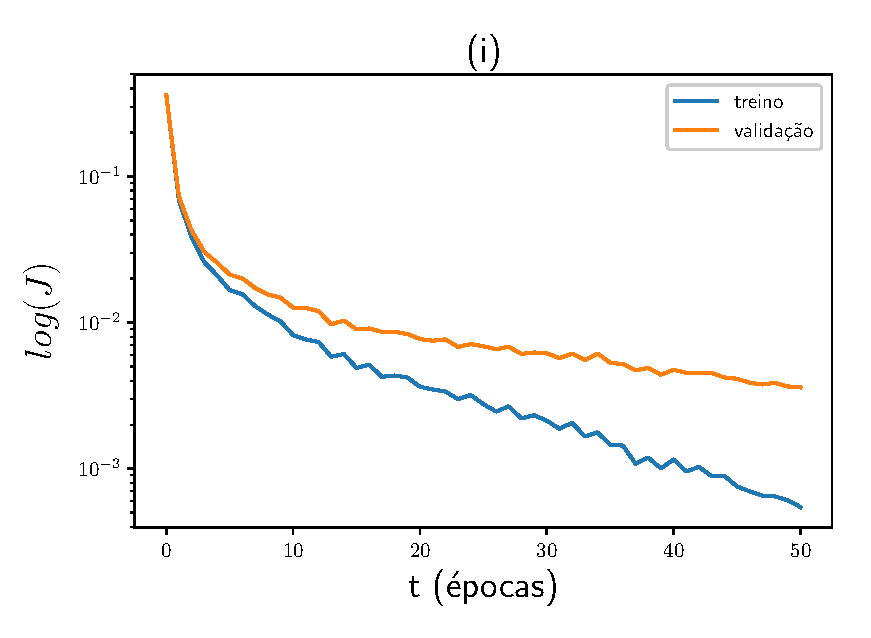
\includegraphics[width=0.98\linewidth]{figuras/C5o6C5o12C5o36C5o36Rfl100MchD_loss.eps}
		\end{subfigure}\hfill%
		\begin{subfigure}{.5\textwidth}
			\centering
			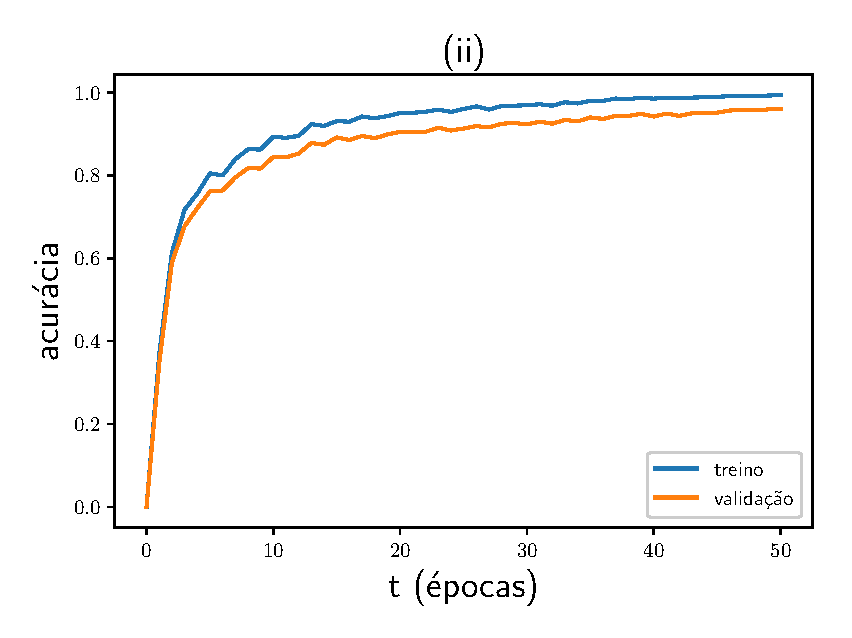
\includegraphics[width=0.95\linewidth]{figuras/C5o6C5o12C5o36C5o36Rfl100MchD_acc.eps}
		\end{subfigure}\hfill%
		\newline
		\begin{subfigure}{.5\textwidth}
			\centering
			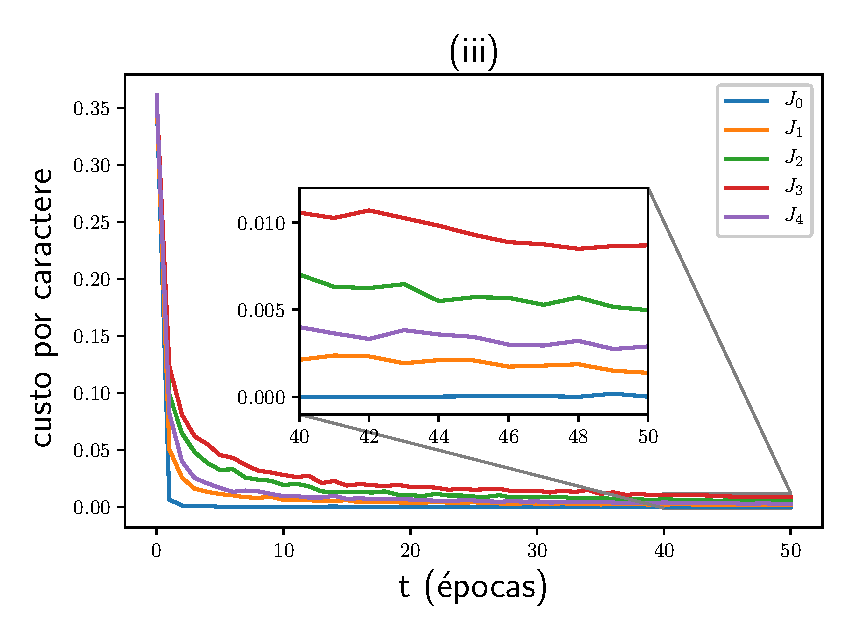
\includegraphics[width=0.95\linewidth]{figuras/C5o6C5o12C5o36C5o36Rfl100MchD_lossi.eps}
		\end{subfigure}\hfill%
		\begin{subfigure}{.5\textwidth}
			\centering
			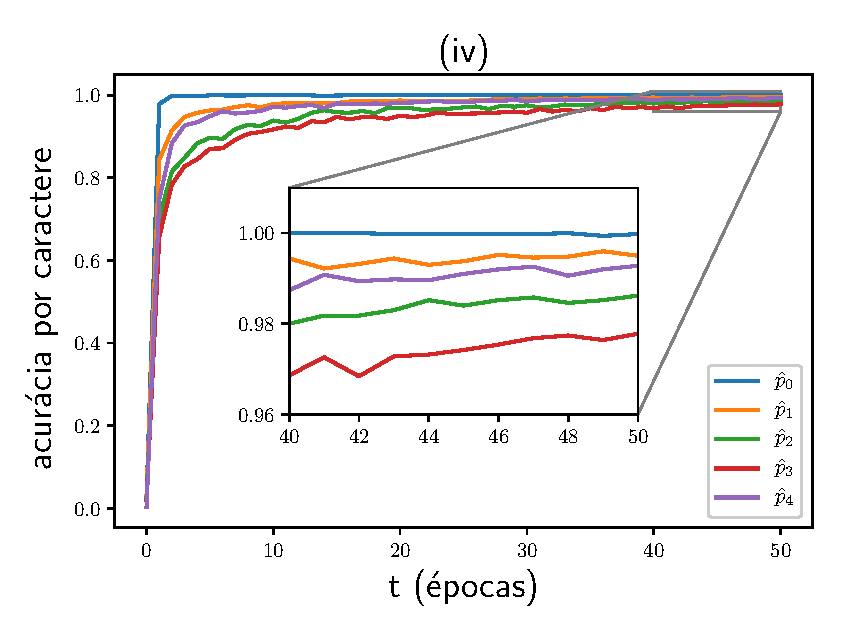
\includegraphics[width=0.95\linewidth]{figuras/C5o6C5o12C5o36C5o36Rfl100MchD_acci.eps}
		\end{subfigure}\hfill%
		\newline
	\end{center}
	\small (i) custo (escala logarítmica) e (ii) acurácia ao longo das épocas para o conjunto de treino e validação. (iii) custo e (iv) acurácia por classificador ao longo das épocas para o conjunto de validação.  
\end{figure}
 


